\let\negmedspace\undefined
\let\negthickspace\undefined
\documentclass[journal]{IEEEtran}
\usepackage[a5paper, margin=10mm, onecolumn]{geometry}
\usepackage{lmodern} 
\usepackage{tfrupee} 

\setlength{\headheight}{1cm} 
\setlength{\headsep}{0mm}     

\usepackage{gvv-book}
\usepackage{gvv}
\usepackage{cite}
\usepackage{amsmath,amssymb,amsfonts,amsthm}
\usepackage{algorithmic}
\usepackage{graphicx}
\usepackage{textcomp}
\usepackage{xcolor}
\usepackage{txfonts}
\usepackage{listings}
\usepackage{enumitem}
\usepackage{mathtools}
\usepackage{gensymb}
\usepackage{comment}
\usepackage{multicol}
\usepackage[breaklinks=true]{hyperref}
\usepackage{tkz-euclide} 
\usepackage{listing}

\graphicspath{ {./figs/} }

\begin{document}


\title{
ASSIGNMENT 4: GATE 2019 \\
IN:INSTRUMENTATION ENGINEERING}
\author{AI25BTECH11013-Gautham Pocha}
\maketitle
\renewcommand{\thefigure}{\theenumi}
\renewcommand{\thetable}{\theenumi} 

\begin{enumerate}
\item The fishermen, \_\_\_\_\_ the flood victims owed their lives, were rewarded by the government.
\begin{multicols}{4}
\begin{enumerate}
\item whom
\item to which
\item to whom
\item that
\end{enumerate}
\end{multicols} \hfill(GATE IN 2019)

\item Some students were not involved in the strike. If the above statement is true, which of the following conclusions is/are logically necessary?
\begin{enumerate}
\item Some who were involved in the strike were students.
\item No student was involved in the strike.
\item At least one student was involved in the strike.
\item Some who were not involved in the strike were students.
\end{enumerate}
\begin{multicols}{4}
\begin{enumerate}
\item 1 and 2
\item 3
\item 4
\item 2 and 3
\end{enumerate}
\end{multicols} \hfill(GATE IN 2019)

\item The radius as well as the height of a circular cone increases by 10\%. The percentage increase in its volume is \_\_\_\_\_.
\begin{multicols}{4}
\begin{enumerate}
\item 17.1
\item 21.0
\item 33.1
\item 72.8
\end{enumerate}
\end{multicols} \hfill(GATE IN 2019)

\item Five numbers 10, 7, 5, 4 and 2 are to be arranged in a sequence from left to right following the directions given below:
\begin{enumerate}
\item No two odd or even numbers are next to each other.
\item The second number from the left is exactly half of the left-most number.
\item The middle number is exactly twice the right-most number.
\end{enumerate}
Which is the second number from the right?
\begin{multicols}{4}
\begin{enumerate}
\item 2
\item 4
\item 7
\item 10
\end{enumerate}
\end{multicols} \hfill(GATE IN 2019)

\item Until Iran came along, India had never been \_\_\_\_\_ in kabaddi.
\begin{multicols}{4}
\begin{enumerate}
\item defeated
\item defeating
\item defeat
\item defeatist
\end{enumerate}
\end{multicols} \hfill(GATE IN 2019)

\item Since the last one year, after a 125 basis point reduction in repo rate by the Reserve Bank of India, banking institutions have been making a demand to reduce interest rates on small saving schemes. Finally, the government announced yesterday a reduction in interest rates on small saving schemes to bring them on par with fixed deposit interest rates. Which one of the following statements can be inferred from the given passage?
\begin{enumerate}
\item Whenever the Reserve Bank of India reduces the repo rate, the interest rates on small saving schemes are also reduced
\item Interest rates on small saving schemes are always maintained on par with fixed deposit interest rates
\item The government sometimes takes into consideration the demands of banking institutions before reducing the interest rates on small saving schemes
\item A reduction in interest rates on small saving schemes follow only after a reduction in repo rate by the Reserve Bank of India
\end{enumerate}
 \hfill(GATE IN 2019)

\item In a country of 1400 million population, 70\% own mobile phones. Among the mobile phone owners, only 294 million access the Internet. Among these Internet users, only half buy goods from e-commerce portals. What is the percentage of these buyers in the country?
\begin{multicols}{4}
\begin{enumerate}
\item 10.50
\item 14.70
\item 15.00
\item 50.00
\end{enumerate}
\end{multicols} \hfill(GATE IN 2019)

\item The nomenclature of Hindustani music has changed over the centuries. Since the medieval period dhrupad styles were identified as baanis. Terms like gayaki and baaj were used to refer to vocal and instrumental styles, respectively. With the institutionalization of music education the term gharana became acceptable. Gharana originally referred to hereditary musicians from a particular lineage, including disciples and grand disciples. Which one of the following pairings is NOT correct?
\begin{enumerate}
\item dhrupad, baani
\item gayaki, vocal
\item baaj, institution
\item gharana, lineage
\end{enumerate}
\hfill(GATE IN 2019)

\item Two trains started at 7AM from the same point. The first train travelled north at a speed of 80km/h and the second train travelled south at a speed of 100 km/h. The time at which they were 540 km apart is \_\_\_\_\_ AM.
\begin{multicols}{4}
\begin{enumerate}
\item 9
\item 10
\item 11
\item 11.30
\end{enumerate}
\end{multicols} \hfill(GATE IN 2019)

\item ``I read somewhere that in ancient times the prestige of a kingdom depended upon the number of taxes that it was able to levy on its people. It was very much like the prestige of a head-hunter in his own community.'' Based on the paragraph above, the prestige of a head-hunter depended upon
\begin{enumerate}
\item the prestige of the kingdom
\item the prestige of the heads
\item the number of taxes he could levy
\item the number of heads he could gather
\end{enumerate}
\hfill(GATE IN 2019)

\item $\vec{a}, \vec{b}, \vec{c}$ are three orthogonal vectors. Given that $\vec{a} = \hat{i} + 2\hat{j} + 5\hat{k}$ and $\vec{b} = \hat{i} + 2\hat{j} - \hat{k}$, the vector $\vec{c}$ is parallel to
\begin{multicols}{4}
\begin{enumerate}
\item $\hat{i} + 2\hat{j} + 3\hat{k}$
\item $2\hat{i} + \hat{j}$
\item $2\hat{i} - \hat{j}$
\item $4\hat{k}$
\end{enumerate}
\end{multicols} \hfill(GATE IN 2019)

\item The vector function $\vec{A}$ is given by $\vec{A} = \nabla u$, where $u(x, y)$ is a scalar function. Then $|\nabla \times \vec{A}|$ is
\begin{multicols}{4}
\begin{enumerate}
\item $-1$
\item $0$
\item $1$
\item $\infty$
\end{enumerate}
\end{multicols} \hfill(GATE IN 2019)

\item A box has 8 red balls and 8 green balls. Two balls are drawn randomly in succession from the box without replacement. The probability that the first ball drawn is red and the second ball drawn is green is
\begin{multicols}{4}
\begin{enumerate}
\item $4/15$
\item $7/16$
\item $1/2$
\item $8/15$
\end{enumerate}
\end{multicols} \hfill(GATE IN 2019)

\item In the Figures (a) and (b) shown below, the transformers are identical and ideal, except that the transformer in Figure (b) is centre-tapped. Assuming ideal diodes, the ratio of the root-mean-square (RMS) voltage across the resistor $R$ in Figure (a) to that in Figure (b) is

\begin{figure}[H]
    \centering
    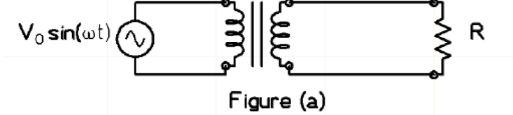
\includegraphics[width=0.6\textwidth]{1.png}
    \caption{}
    \label{fig:fig1}
\end{figure}

\begin{figure}[H]
    \centering
    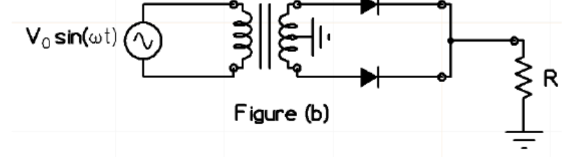
\includegraphics[width=0.6\textwidth]{2.png}
    \caption{}
    \label{fig:fig2}
\end{figure}

\begin{multicols}{4}
\begin{enumerate}
\item $\sqrt{2}:1$
\item $2:1$
\item $2\sqrt{2}:1$
\item $4:1$
\end{enumerate}
\end{multicols} \hfill(GATE IN 2019)

\item The output $y(t)$ of a system is related to its input $x(t)$ as
$y(t) = \int_{0}^{t} x(\tau-2)dt,$
where, $x(t) = 0$ and $y(t) = 0$ for $t \leq 0$. The transfer function of the system is
\begin{multicols}{2}
\begin{enumerate}
\item $\frac{1}{s}$
\item $\frac{(1-e^{-2s})}{s}$
\item $\frac{e^{-2s}}{s}$
\item $\frac{1}{s} - e^{-2s}$
\end{enumerate}
\end{multicols} \hfill(GATE IN 2019)

\item The input $x[n]$ and output $y[n]$ of a discrete-time system are related as $y[n] = \alpha y[n - 1] + x[n]$. The condition on $\alpha$ for which the system is Bounded-Input Bounded-Output (BIBO) stable is
\begin{multicols}{4}
\begin{enumerate}
\item $|\alpha| < 1$
\item $|\alpha| = 1$
\item $|\alpha| > 1$
\item $|\alpha| < 3/2$
\end{enumerate}
\end{multicols} \hfill(GATE IN 2019)

\item In a cascade control system, the closed loop transfer function of the inner loop may be assumed to have a single time-constant $\tau_1$. Similarly, the closed loop transfer function of the outer loop may be assumed to have a single time-constant $\tau_2$. The desired relationship between $\tau_1$ and $\tau_2$ in a well-designed control system is
\begin{enumerate}
\item $\tau_1$ is much less than $\tau_2$
\item $\tau_1$ is equal to $\tau_2$
\item $\tau_1$ is much greater than $\tau_2$
\item $\tau_1$ is independent of $\tau_2$
\end{enumerate}
 \hfill(GATE IN 2019)

\item The loop-gain function $L(s)$ of a control system with unity feedback is given to be
$L(s) = \frac{k}{(s+1)(s+2)(s+3)}, \text{ where } k > 0.$
If the gain cross-over frequency of the loop-gain function is less than its phase cross-over frequency, the closed-loop system is
\begin{enumerate}
\item unstable
\item marginally stable
\item conditionally stable
\item stable
\end{enumerate}
 \hfill(GATE IN 2019)

\item If each of the values of inductance, capacitance and resistance of a series LCR circuit are doubled, the Q-factor of the circuit would

\begin{enumerate}
\item reduce by a factor $\sqrt{2}$
\item reduce by a factor 2
\item increase by a factor $\sqrt{2}$
\item increase by a factor 2
\end{enumerate}
\hfill(GATE IN 2019)

\item In the circuit shown below, the input voltage $V_{in}$ is positive. The current (I) - voltage (V) characteristics of the diode can be assumed to be $I = I_0 e^{V/V_T}$ under the forward bias condition, where $V_T$ is the thermal voltage and $I_0$ is the reverse saturation current. Assuming an ideal op-amp, the output voltage $V_{out}$ of the circuit is proportional to
\begin{figure}[H]
    \centering
    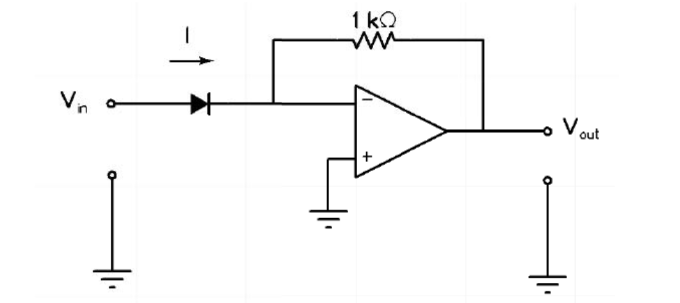
\includegraphics[width=0.6\textwidth]{3.png}
    \caption{}
    \label{fig:fig3}
\end{figure}
\begin{multicols}{4}
\begin{enumerate}
\item $\log_e(V_{in}/V_T)$
\item $2V_{in}$
\item $e^{V_{in}/V_T}$
\item $V^2_{in}$
\end{enumerate}
\end{multicols} \hfill(GATE IN 2019)

\item The correct biasing conditions for typical operation of light emitting diodes, photodiodes, Zener diodes are, respectively

\begin{enumerate}
\item forward bias, reverse bias, reverse bias
\item reverse bias, reverse bias, forward bias
\item forward bias, forward bias, reverse bias
\item reverse bias, forward bias, reverse bias
\end{enumerate}
 \hfill(GATE IN 2019)

\item The circuit shown in the figure below uses ideal positive edge-triggered synchronous J-K flip flops with outputs X and Y. If the initial state of the output is X=0 and Y=0 just before the arrival of the first clock pulse, the state of the output just before the arrival of the second clock pulse is
\begin{figure}[H]
    \centering
    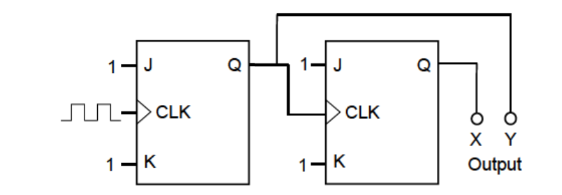
\includegraphics[width=0.6\textwidth]{4.png}
    \caption{}
    \label{fig:fig4}
\end{figure}
\begin{multicols}{2}
\begin{enumerate}
\item X=0, Y=0
\item X=0, Y=1
\item X=1, Y=0
\item X=1, Y=1
\end{enumerate}
\end{multicols} \hfill(GATE IN 2019)

\item Thermocouples measure temperature based on
\begin{multicols}{2}
\begin{enumerate}
\item Photoelectric effect
\item Seebeck effect
\item Hall effect
\item Thermal expansion
\end{enumerate}
\end{multicols} \hfill(GATE IN 2019)

\item Four strain gauges in a Wheatstone bridge configuration are connected to an instrumentation amplifier as shown in the figure. From the choices given below, the preferred value for the common mode rejection ratio (CMRR) of the amplifier, in dB, would be
\begin{figure}[H]
    \centering
    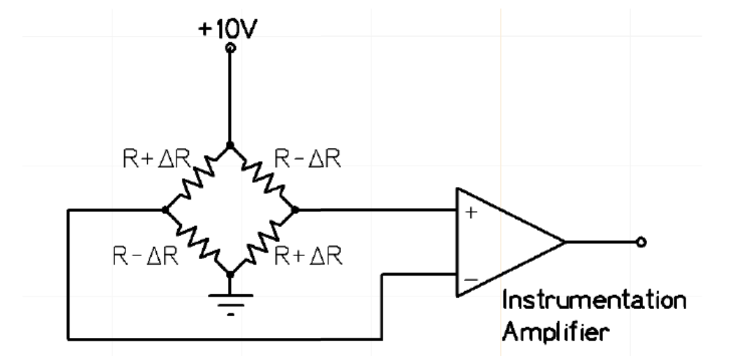
\includegraphics[width=0.6\textwidth]{5.png}
    \caption{}
    \label{fig:fig5}
\end{figure}
\begin{multicols}{4}
\begin{enumerate}
\item $-20$
\item $0$
\item $3$
\item $100$
\end{enumerate}
\end{multicols} \hfill(GATE IN 2019)

\item In a single-mode optical fiber, the zero-dispersion wavelength refers to the wavelength at which the
\begin{enumerate}
\item material dispersion is zero.
\item waveguide dispersion is zero.
\item sum of material dispersion and waveguide dispersion is zero.
\item material dispersion and waveguide dispersion are simultaneously zero.
\end{enumerate}
 \hfill(GATE IN 2019)

\item A $3 \times 3$ matrix has eigenvalues 1, 2 and 5. The determinant of the matrix is \_\_\_\_\_.
\hfill(GATE IN 2019)
\item In the circuit shown below, maximum power is transferred to the load resistance $R_L$, when $R_L = $ \_\_\_\_\_ $\Omega$.
\begin{figure}[H]
    \centering
    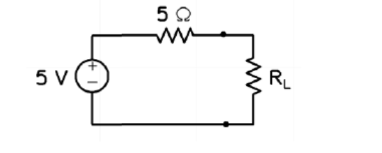
\includegraphics[width=0.6\textwidth]{6.png}
    \caption{}
    \label{fig:fig6}
\end{figure}
\hfill(GATE IN 2019)
\item Consider a circuit comprising only resistors with constant resistance and ideal independent DC voltage sources. If all the resistances are scaled down by a factor 10, and all source voltages are scaled up by a factor 10, the power dissipated in the circuit scales up by a factor of \_\_\_\_\_.
\hfill(GATE IN 2019)
\item In the circuit shown below, initially the switch $S_1$ is open, the capacitor C1 has a charge of 6 coulomb, and the capacitor C2 has 0 coulomb. After $S_1$ is closed, the charge on C2 in steady state is \_\_\_\_\_ coulomb.
\begin{figure}[H]
    \centering
    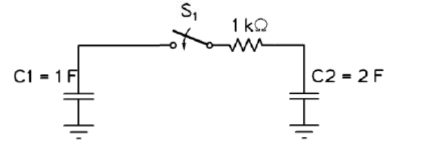
\includegraphics[width=0.6\textwidth]{7.png}
    \caption{}
    \label{fig:fig7}
\end{figure}
\hfill(GATE IN 2019)

\item An 8-bit weighted resistor digital-to-analog converter (DAC) has the smallest resistance of 500 $\Omega$. The largest resistance has a value \_\_\_\_\_ $k\Omega$.
\hfill(GATE IN 2019)
\item The total number of Boolean functions with distinct truth-tables that can be defined over 3 Boolean variables is \_\_\_\_\_.
\hfill(GATE IN 2019)
\item The figure below shows the $i^{th}$ full-adder block of a binary adder circuit. $C_i$ is the input carry and $C_{i+1}$ is the output carry of the circuit. Assume that each logic gate has a delay of 2 nanosecond, with no additional time delay due to the interconnecting wires. If the inputs $A_i$, $B_i$ are available and stable throughout the carry propagation, the maximum time taken for an input $C_i$ to produce a steady-state output $C_{i+1}$ is \_\_\_\_\_ nanosecond.
\begin{figure}[H]
    \centering
    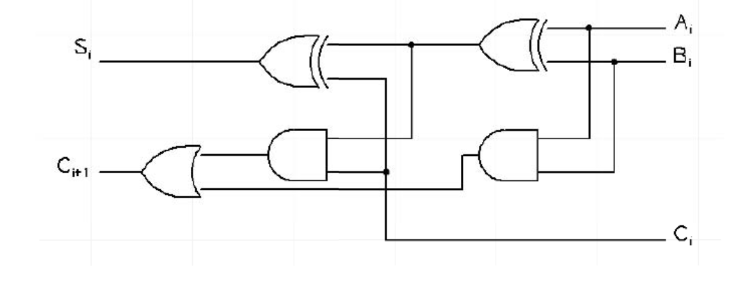
\includegraphics[width=0.6\textwidth]{8.png}
    \caption{}
    \label{fig:fig8}
\end{figure}
\hfill(GATE IN 2019)
\item The resistance of a resistor is measured using a voltmeter and an ammeter. The voltage measurements have a mean value of 1V and standard deviation of 0.12 V while current measurements have a mean value of 1 mA with standard deviation of 0.05 mA. Assuming that the errors in voltage and current measurements are independent, the standard deviation of the calculated resistance value is \_\_\_\_\_ $\Omega$.
\hfill(GATE IN 2019)
\item A pitot-static tube is used to estimate the velocity of an incompressible fluid of density 1 kg/m$^3$. If the pressure difference measured by the tube is 200 N/m$^2$, the velocity of the fluid, assuming the pitot-tube coefficient to be 1.0, is \_\_\_\_\_ m/s.
\hfill(GATE IN 2019)
\item A signal $\cos(2\pi f_m t)$ modulates a carrier $\cos(2\pi f_c t)$ using the double-sideband-with-carrier (DSBWC) scheme to yield a modulated signal $\cos(2\pi f_c t)+0.3\cos(2\pi f_m t)\cos(2\pi f_c t)$. The modulation index is \_\_\_\_\_. (Answer should be rounded off to one decimal place)
\hfill(GATE IN 2019)
\item The curve $y=f(x)$ is such that the tangent to the curve at every point $(x,y)$ has a Y-axis intercept $c$, given by $c=-y$. Then, $f(x)$ is proportional to
\begin{multicols}{4}
\begin{enumerate}
\item $x^{-1}$
\item $x^2$
\item $x^3$
\item $x^4$
\end{enumerate}
\end{multicols} \hfill(GATE IN 2019)

\item The function $p(x)$ is given by $p(x)=A/x^\mu$ where $A$ and $\mu$ are constants with $\mu>1$ and $1\leq x<\infty$ and $p(x)=0$ for $-\infty<x<1$. For $p(x)$ to be a probability density function, the value of $A$ should be equal to
\begin{multicols}{2}
\begin{enumerate}
\item $\mu-1$
\item $\mu+1$
\item $1/(\mu-1)$
\item $1/(\mu+1)$
\end{enumerate}
\end{multicols} \hfill(GATE IN 2019)
\item The dynamics of the state $\myvec{ x_1 \\ x_2 }$ of a system is governed by the differential equation
$\myvec{ \dot{x}_1 \\ \dot{x}_2 } = 
\myvec{ 1 & 2 \\ -3 & -4 }
\myvec{ x_1 \\ x_2 } + 
\myvec{ 20 \\ 10 }$
Given that the initial state is $\myvec{ 0 \\ 0 }$, the steady state value of $\myvec{ x_1 \\ x_2 }$ is
\begin{multicols}{4}
\begin{enumerate}
\item $\myvec{ -30 \\ -40 }$
\item $\myvec{ -20 \\ -10 }$
\item $\myvec{ 5 \\ -15 }$
\item $\myvec{ 50 \\ -35 }$
\end{enumerate}
\end{multicols} \hfill(GATE IN 2019)

\item A complex function $f(z) = u(x, y) + i \, v(x, y)$ and its complex conjugate $f^*(z) = u(x, y) - i \, v(x, y)$ are both analytic in the entire complex plane, where $z = x + i \, y$ and $i = \sqrt{-1}$. The function $f$ is then given by
\begin{multicols}{2}
\begin{enumerate}
\item $f(z) = x + i \, y$
\item $f(z) = x^2 - y^2 + i \, 2xy$
\item $f(z) = \text{constant}$
\item $f(z) = x^2 + y^2$
\end{enumerate}
\end{multicols} \hfill(GATE IN 2019)

\item In a control system with unity gain feedback, the plant has the transfer function $P(s) = 3/s$. Assuming that a controller of the form $C(s) = K/(s + p)$ is used, where $K$ is a positive constant, the value of $p$ for which the root-locus of the closed-loop system passes through the points $-3 \pm j3\sqrt{3}$ where $j = \sqrt{-1}$, is
\begin{multicols}{4}
\begin{enumerate}
\item 3
\item $3\sqrt{3}$
\item 6
\item 9
\end{enumerate}
\end{multicols} \hfill(GATE IN 2019)

\item The forward path transfer function $L(s)$ of the control system shown in Figure (a) has the asymptotic Bode plot shown in Figure (b). If the disturbance $d(t)$ is given by $d(t) = 0.1 \sin(\omega t)$ where $\omega = 5 \, rad/s$, the steady-state amplitude of the output $y(t)$ is
\begin{multicols}{2}
\begin{figure}[H]
    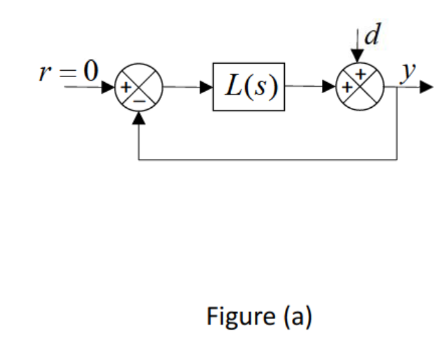
\includegraphics[width=0.3\textwidth]{9.png}
    \caption{}
    \label{fig:fig9}
\end{figure}
\begin{figure}[H]
    \centering
    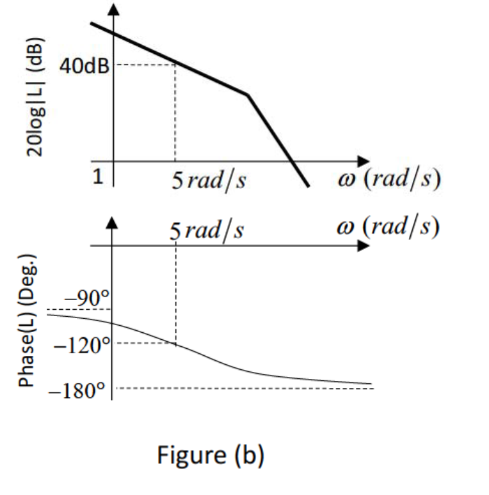
\includegraphics[width=0.3\textwidth]{10.png}
    \caption{}
    \label{fig:fig10}
\end{figure}
\end{multicols}
\begin{multicols}{2}
\begin{enumerate}
\item $1.00 \times 10^{-3}$
\item $2.50 \times 10^{-3}$
\item $5.00 \times 10^{-3}$
\item $10.00 \times 10^{-3}$
\end{enumerate}
\end{multicols} \hfill(GATE IN 2019)

\item In the control system shown in the figure below, a reference signal $r(t) = t^2$ is applied at time $t = 0$. The control system employs a PID controller $C(s) = K_P + K_I / s + K_D s$ and the plant has a transfer function $P(s) = 3 / s$. If $K_P = 10$, $K_I = 1$ and $K_D = 2$, the steady state value of $e$ is
\begin{figure}[H]
    \centering
    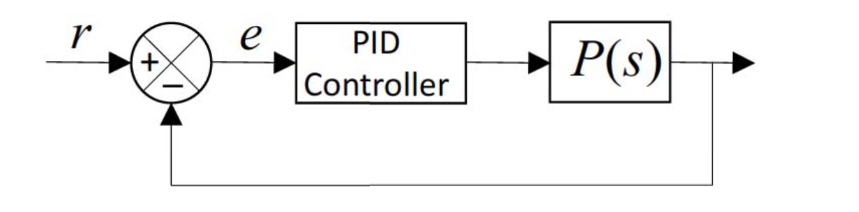
\includegraphics[width=0.6\textwidth]{11.png}
    \caption{}
    \label{fig:fig11}
\end{figure}
\begin{multicols}{4}
\begin{enumerate}
\item 0
\item 2/3
\item 1
\item $\infty$
\end{enumerate}
\end{multicols} \hfill(GATE IN 2019)

\item A voltage amplifier is constructed using enhancement mode MOSFETs labeled M1, M2, M3 and M4 in the figure below. M1, M2 and M4 are n-channel MOSFETs and M3 is a p-channel MOSFET. All MOSFETs operate in saturation mode and channel length modulation can be ignored. The low frequency, small signal input and output voltages are $v_{in}$ and $v_{out}$ respectively and the dc power supply voltage is $V_{DD}$. All n-channel MOSFETs have identical transconductance $g_{mn}$ while the p-channel MOSFET has transconductance $g_{mp}$. The expressions for the low frequency small signal voltage gain $v_{out}/v_{in}$ is
\begin{figure}[H]
    \centering
    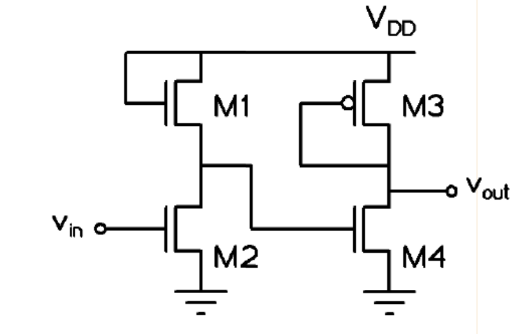
\includegraphics[width=0.6\textwidth]{12.png}
    \caption{}
    \label{fig:fig12}
\end{figure}
\begin{enumerate}
\item $-g_{mn}/g_{mp}$
\item $-g_{mn}(g_{mn} + g_{mp})^{-1}$
\item $+g_{mn}/g_{mp}$
\item $g_{mn}(g_{mn} + g_{mp})^{-1}$
\end{enumerate}
 \hfill(GATE IN 2019)

\item In the circuit shown below, assume that the comparators are ideal and all components have zero propagation delay. In one period of the input signal $V_{in} = 6 \sin(\omega t)$, the fraction of the time for which the output OUT is in logic state HIGH is
\begin{figure}[H]
    \centering
    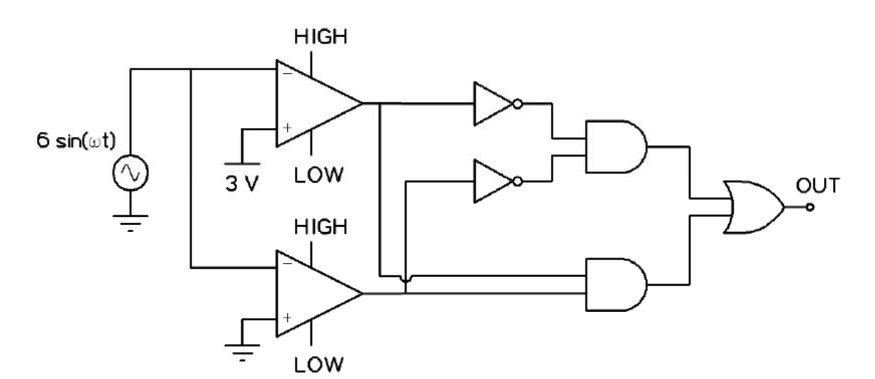
\includegraphics[width=0.6\textwidth]{13.png}
    \caption{}
    \label{fig:fig13}
\end{figure}
\begin{multicols}{4}
\begin{enumerate}
\item 1/12
\item 1/2
\item 2/3
\item 5/6
\end{enumerate}
\end{multicols} \hfill(GATE IN 2019)

\item $X = X_1X_0$ and $Y = Y_1Y_0$ are 2-bit binary numbers. The Boolean function $S$ that satisfies the condition ``If $X > Y$, then $S = 1$'', in its minimized form, is
\begin{enumerate}
\item $X_1Y_1 + X_0Y_0$
\item $X_1\overline{Y}_1 + X_0\overline{Y}_0\overline{Y}_1 + X_0\overline{Y}_0X_1$
\item $X_1\overline{Y}_1X_0\overline{Y}_0$
\item $X_1Y_1 + X_0\overline{Y}_0Y_1 + X_0\overline{Y}_0X_1$
\end{enumerate}
 \hfill(GATE IN 2019)

\item In the circuit below, the light dependent resistor (LDR) receives light from the LED. The LDR has resistances of 5 k$\Omega$ and 500 $\Omega$ under dark and illuminated conditions, respectively. The LED is OFF at time $t < 0$. At time $t = 0 \, \text{s}$, the switch $S_1$ is closed for 1 ms and then kept open thereafter. Assuming zero propagation delay in the devices, the LED
\begin{figure}[H]
    \centering
    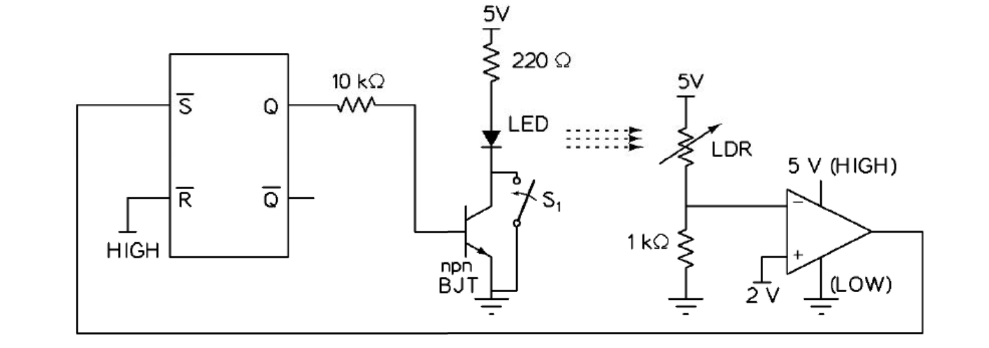
\includegraphics[width=0.6\textwidth]{14.png}
    \caption{}
    \label{fig:fig14}
\end{figure}
\begin{enumerate}
\item turns ON when $S_1$ is closed and remains ON after $S_1$ is opened
\item turns ON when $S_1$ is closed and turns OFF after $S_1$ is opened
\item turns ON when $S_1$ is closed and toggles periodically from ON to OFF after $S_1$ is opened
\item remains OFF when $S_1$ is closed and continues to remain OFF after $S_1$ is opened
\end{enumerate}
\hfill(GATE IN 2019)

\item A differential capacitive sensor with a distance between the extreme plates 100 mm is shown in figure below. The difference voltage $\Delta V = V_1 - V_2$, where $V_1$ and $V_2$ are the rms values, for a downward displacement of 10 mm of the intermediate plate from the central position, in volts, is
\begin{figure}[H]
    \centering
    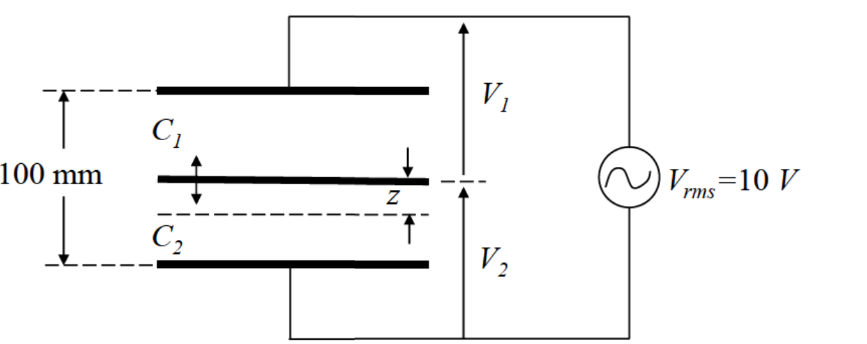
\includegraphics[width=0.6\textwidth]{15.png}
    \caption{}
    \label{fig:fig15}
\end{figure}
\begin{multicols}{4}
\begin{enumerate}
\item 0.9
\item 1.0
\item 1.1
\item 2
\end{enumerate}
\end{multicols} \hfill(GATE IN 2019)

\item A piezoelectric transducer with sensitivity of 30 mV/kPa is intended to be used in the range of 0 kPa to 100 kPa. The readout circuit has a peak noise amplitude of 0.3 mV and measured signals over the full pressure range are encoded with 10 bits. The smallest pressure that produces a non-zero output, in units of Pa, is approximately
\begin{multicols}{4}
\begin{enumerate}
\item 10
\item 100
\item 240
\item 300
\end{enumerate}
\end{multicols} \hfill(GATE IN 2019)

\item A 100 W light source emits uniformly in all directions. A photodetector having a circular active area whose diameter is 2 cm is placed 1 m away from the source, normal to the incident light. If the responsivity of the photodetector is 0.4 A/W, the photo-current generated in the detector, in units of mA, is
\begin{multicols}{4}
\begin{enumerate}
\item 1
\item 4
\item 100
\item 400
\end{enumerate}
\end{multicols} \hfill(GATE IN 2019)

\item A resistance-meter has five measurement range-settings between 200 $\Omega$ and 2 M$\Omega$ in multiples of 10. The meter measures resistance of a device by measuring a full-range voltage of 2 V across the device by passing an appropriate constant current for each range-setting. If a device having a resistance value in the range 8 k$\Omega$ to 12 k$\Omega$ and a maximum power rating of 100 $\mu$W is to be measured safely with this meter, the choice for range-setting on the meter for best resolution in measurement, in k$\Omega$, is
\begin{multicols}{4}
\begin{enumerate}
\item 2
\item 20
\item 200
\item 2000
\end{enumerate}
\end{multicols} \hfill(GATE IN 2019)

\item A pulsed laser emits rectangular pulses of width 1 nanosecond at a repetition rate of 1 kHz. If the average power output is 1 mW, the average power over a single pulse duration, in watts, is
\begin{multicols}{4}
\begin{enumerate}
\item 1
\item 10
\item 100
\item 1000
\end{enumerate}
\end{multicols} \hfill(GATE IN 2019)

\item Four identical resistive strain gauges with gauge factor of 2.0 are used in a Wheatstone bridge as shown in the figure below. Only one of the strain gauges $R_{SENSE}$ changes its resistance due to strain. If the output voltage $V_{OUT}$ is measured to be 1 mV, the magnitude of strain, in units of microstrain, is
\begin{figure}[H]
    \centering
    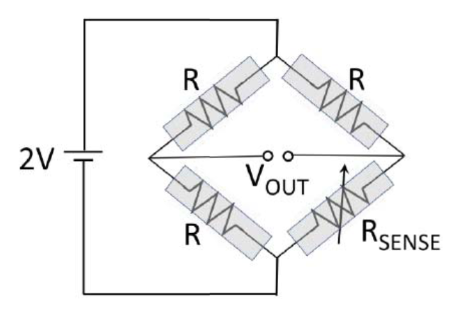
\includegraphics[width=0.6\textwidth]{16.png}
    \caption{}
    \label{fig:fig16}
\end{figure}
\begin{enumerate}
\item 1
\item 10
\item 100
\item 1000
\end{enumerate}
\hfill(GATE IN 2019)

\item The frequency response of a digital filter $H(\omega)$ has the following characteristics: Passband: $0.95 \leq |H(\omega)| \leq 1.05$ for $0 \leq \omega \leq 0.3\pi$ and Stopband: $0 \leq |H(\omega)| \leq 0.005$ for $0.4\pi \leq \omega \leq \pi$, where $\omega$ is the normalized angular frequency in rad/sample. If the analog upper cut off frequency for the passband of the above digital filter is to be 1.2 kHz, then the sampling frequency should be \_\_\_\_\_ kHz.
\hfill(GATE IN 2019)
\item In the circuit shown below, a step input voltage of magnitude 5 V is applied at node A at time $t = 0$. If the capacitor has no charge for $t \leq 0$, the voltage at node P at $t = 6 \, \mu s$ is \_\_\_\_\_ V. (Answer should be rounded off to two decimal places)
\begin{figure}[H]
    \centering
    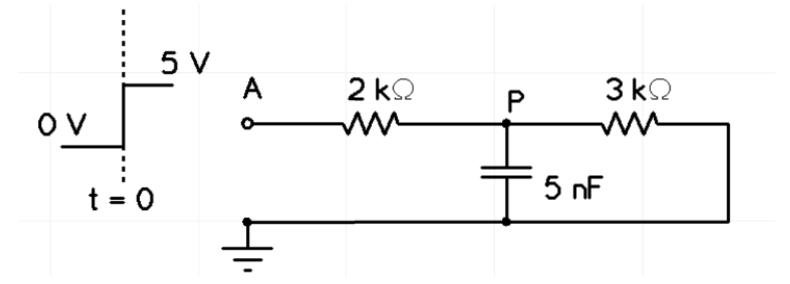
\includegraphics[width=0.6\textwidth]{17.png}
    \caption{}
    \label{fig:fig17}
\end{figure}
\hfill(GATE IN 2019)
\item In the circuit shown below, the angular frequency $\omega$ at which the current is in phase with the voltage is \_\_\_\_\_ rad/s.
\begin{figure}[H]
    \centering
    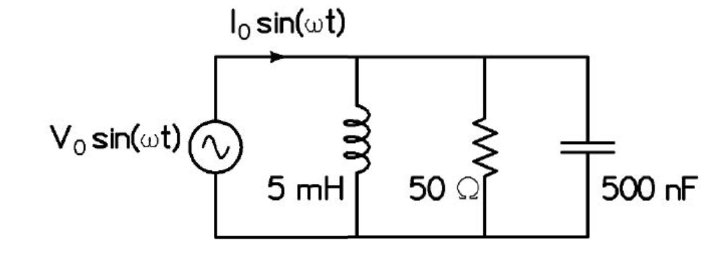
\includegraphics[width=0.6\textwidth]{18.png}
    \caption{}
    \label{fig:fig18}
\end{figure}
\hfill(GATE IN 2019)
\item The transfer function relating the input $x(t)$ to the output $y(t)$ of a system is given by $G(s) = 1/(s + 3)$. A unit-step input is applied to the system at time $t = 0$. Assuming that $y(0) = 3$, the value of $y(t)$ at time $t = 1$ is \_\_\_\_\_ (Answer should be rounded off to two decimal places)
\hfill(GATE IN 2019)
\item The output of a continuous-time system $y(t)$ is related to its input $x(t)$ as
$ y(t) = x(t) + \frac{1}{2}x(t - 1). $
If the Fourier transforms of $x(t)$ and $y(t)$ are $X(\omega)$ and $Y(\omega)$ respectively, and $|X(0)|^2 = 4$, the value of $|Y(0)|^2$ is \_\_\_\_\_.
\hfill(GATE IN 2019)
\item A discrete-time signal $x[n] = e^{j(\frac{5\pi}{3})n} + e^{j(\frac{\pi}{4})n}$ is down-sampled to the signal $x_d[n]$ such that $x_d[n] = x[4n]$. The fundamental period of the down-sampled signal $x_d[n]$ is \_\_\_\_\_.
\hfill(GATE IN 2019)
\item In a control system with unity gain feedback, the transfer function of the loop-gain function is 
$ L(S) = 9e^{-0.1S}/S. $
The phase margin of the loop-gain function $L(S)$ is \_\_\_\_\_ degree.
\hfill(GATE IN 2019)
\item In the circuit shown below, all transistors are n-channel enhancement mode MOSFETs. They are identical and are biased to operate in saturation mode. Ignoring channel length modulation, the output voltage $V_{out}$ is \_\_\_\_\_ V.
\begin{figure}[H]
    \centering
    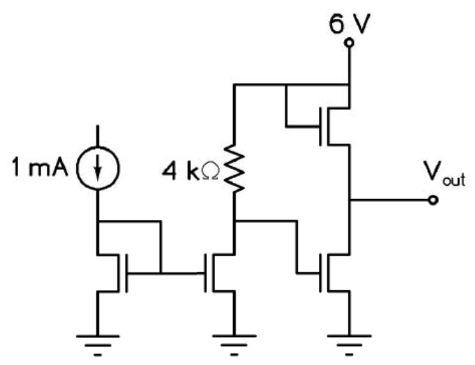
\includegraphics[width=0.6\textwidth]{19.png}
    \caption{}
    \label{fig:fig19}
\end{figure}
\hfill(GATE IN 2019)
\item In the circuit shown below, all OPAMPS are ideal. The current $I = 0 \, A$ when the resistance $R = $ \_\_\_\_\_ k$\Omega$.
\begin{figure}[H]
    \centering
    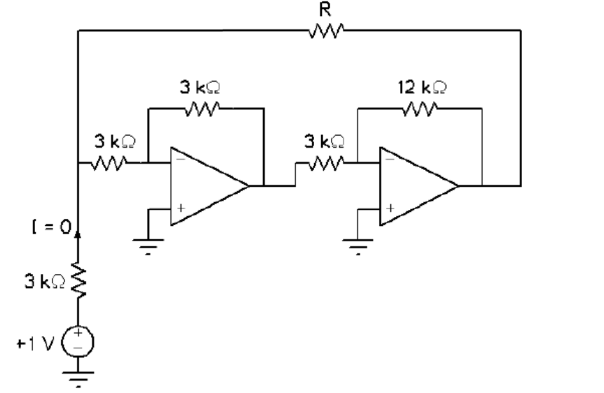
\includegraphics[width=0.6\textwidth]{20.png}
    \caption{}
    \label{fig:fig20}
\end{figure}
\hfill(GATE IN 2019)
\item The parallel resistance-capacitance bridge shown below has a standard capacitance value of $C_1=0.1 \mu F$ and a resistance value of $R_3=10 \, \text{k}\Omega$. The bridge is balanced at a supply frequency of 100 Hz for $R_1=375 \, \text{k}\Omega$, $R_3=10 \, \text{k}\Omega$ and $R_4=14.7 \, \text{k}\Omega$. The value of the dissipation factor $D = 1/(\omega R_p C_p)$ of the parallel combination of $C_p$ and $R_p$ is \_\_\_\_\_. (Answer should be rounded off to THREE decimal places)
\begin{figure}[H]
    \centering
    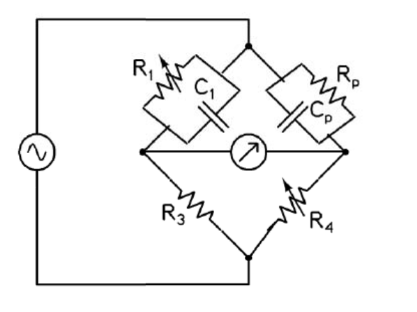
\includegraphics[width=0.6\textwidth]{21.png}
    \caption{}
    \label{fig:fig21}
\end{figure}
\hfill(GATE IN 2019)
\item In a microprocessor with a 16 bit address bus, the most significant address lines A15 to A12 are used to select a 4096 word memory unit, while lines A0 to A11 are used to address a particular word in the memory unit. If the 3 least significant lines of the address bus A0 to A2 are short-circuited to ground, the addressable number of words in the memory unit is \_\_\_\_\_.
\hfill(GATE IN 2019)
\item A signal $x(t)$ has a bandwidth $2B$ about a carrier frequency of $f_c = 2 \, \text{GHz}$ as shown in Figure (a) below. In order to demodulate this signal, it is first mixed (multiplied) with a local oscillator of frequency $f_{LO} = 1.5 \, \text{GHz}$, and then passed through an ideal low-pass filter (LPF) with a cut-off frequency of $2.8 \, \text{GHz}$. The output of the LPF is sent to a digitizer ADC with a sampling rate of $1.6 \, \text{GHz}$ as shown in Figure (b) below. The maximum value of $B$ so that the signal $x(t)$ can be reconstructed from its samples according to the Nyquist sampling theorem is \_\_\_\_\_ MHz.
\begin{figure}[H]
    \centering
    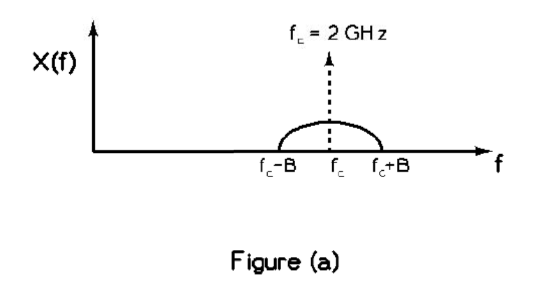
\includegraphics[width=0.6\textwidth]{22.png}
    \caption{}
    \label{fig:fig22}
\end{figure}
\begin{figure}[H]
    \centering
    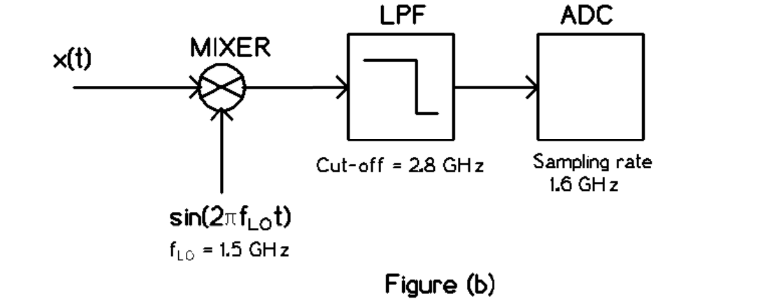
\includegraphics[width=0.6\textwidth]{23.png}
    \caption{}
    \label{fig:fig23}
\end{figure}
\hfill(GATE IN 2019)
\item Consider a Michelson interferometer as shown in the figure below. When the wavelength of the laser light source is switched from 400 nanometer to 500 nanometer, it is observed that the intensity measured at the output port P goes from a minimum to a maximum. This observation is possible when the smallest path difference between the two arms of the interferometer is $\_\_\_\_\_$ nanometer.
\begin{figure}[H]
    \centering
    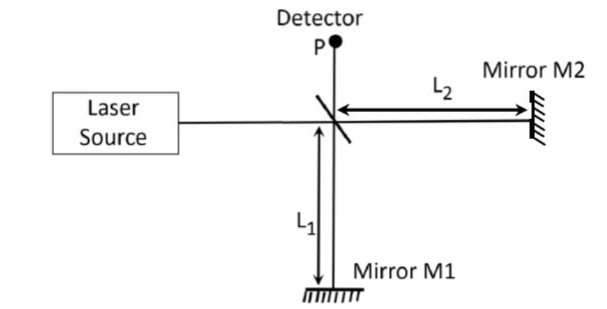
\includegraphics[width=0.6\textwidth]{24.png}
    \caption{}
    \label{fig:fig24}
\end{figure}
\hfill(GATE IN 2019)

\end{enumerate}
\end{document}
